\documentclass{article}
\usepackage{listings}
\usepackage{hyperref}
\usepackage{graphicx}
\usepackage{float}
\usepackage[margin=1.25in]{geometry}
\begin{document}
\title{EOPSY Lab 4 Report}
\author{Krzysztof Rudnicki, 307585}
\date{\today}
\maketitle
\section{Introduction}
\subsection{Page replacement algorithms}
\paragraph{First in First out}
What page replacament algorithm is being used? \\
We use FIFO (First in First out) page replacement algorithm for those laboratories as indicated
by the PageFault.java file line 18
\begin{figure}[H]
\caption{PageFault.java file}
\begin{lstlisting}[language=Java]
[...]
public class PageFault {

  /**
   * The page replacement algorithm for the memory management sumulator.
   * This method gets called whenever a page needs to be replaced.
   * <p>
   * The page replacement algorithm included with the simulator is 
   * FIFO (first-in first-out).  A while or for loop should be used 
   * to search through the current memory contents for a canidate 
   * replacement page.  In the case of FIFO the while loop is used 
   * to find the proper page while making sure that virtPageNum is 
   * not exceeded.
[...]
\end{lstlisting}
\end{figure}
All pages are stored in memory in a queue. Oldest page (First that came in) is
in front of this queue. \\ When we need to replace the page we remove the page that
is first in queue (so the one that came in as a first one, first in, first out)
\\
It is easy to explain and implement but in practical application it performs
poorly. It is still used but usually we use modified version of it.
\cite{Page Replacement Algorithms}
\paragraph{Optimal Page Replacement}
We replace pages which in the future will not be used for the longest time.
This is purely theoretical algorithm. It is perfect but not doable in practice
since operating systems can not know future requests. \\
It is used as a benchmark against which we compare other algorithms. 
\cite{Page Replacement Algorithms}
\paragraph{Least Recently Used}
We replace page which was not used for the longest time. \\
It is based on the idea that we will in future work on pages which we used
heavily in the past. In theory its performance can be close to optimal one but
in practice it is expensive to implement. \\
Most expensive way of implementing this algorithm is using linked lists. Most
recently used pages in front, least recently used in the back. Every time we
reference memory we have to move elements in list which takes a lot of time. \\
We can also use operating system counter \\
This algorithm is often used in different cheaper modified versions.
\cite{Page Replacement Algorithms}
\cite{pageWiki}
\subsection{Other}
\paragraph{Memory Management Unit} 
Hardware unit which translates virtual memory to physical one.
\cite{mmuWiki}
\paragraph{Page fault}
Exception raised when process wants to access page without preparations.
Preparation consists of adding the mapping to process's virtual address space
and/or loading page from a disk. MMU detects the fault but it is up to kernel
and/or loading page from a disk. 

\section{Laboratory}
\subsection{Instruction}
\begin{enumerate}
	\item Map 8 pages of physical memory to the first 8 pages of virtual
		memory
	\item Go through each virtual page and read from one virtual memory
		address 
\end{enumerate}
\subsection{Configuration}
In memory.conf file I changed the memset and mapped first 8 pages of virtual
memory to first 8 pages of physical memory (we could use any physical memory
pages we wanted so I settled for this for sake of simplicity)
\begin{figure}[H]
\caption{memory.conf file}
\begin{lstlisting}
// memset  virt page #  physical page #  R (read from)  
// M (modified) inMemTime (ns) lastTouchTime (ns)
memset 0 0 0 0 0 0
memset 1 1 0 0 0 0
memset 2 2 0 0 0 0
memset 3 3 0 0 0 0
memset 4 4 0 0 0 0
memset 5 5 0 0 0 0
memset 6 6 0 0 0 0
memset 7 7 0 0 0 0

// enable_logging 'true' or 'false'
// When true specify a log_file or leave blank for stdout
enable_logging true

// log_file <FILENAME>
// Where <FILENAME> is the name of the file you want output
// to be print to.
log_file tracefile

// page size, defaults to 2^14 and cannot be greater than 2^26
// pagesize <single page size (base 10)> or <'power' num (base 2)>
pagesize 16384

// addressradix sets the radix 
// in which numerical values are displayed
// 2 is the default value
// addressradix <radix>
addressradix 16

// numpages sets the number of pages (physical and virtual)
// 64 is the default value
// numpages must be at least 2 and no more than 64
// numpages <num>
numpages 64
\end{lstlisting}
\end{figure}
We want to access each virtual page and read from one virtualk memory address of
each page. \\
To achieve this we need to read from pages in increments of pagesize. Which is
set by default to 16384 and I do not change that. \\
We have 64 pages so the last address we will read from will be address 
\[ 64 \cdot 16384 = 1048576 \]
And since we start from address number 0 we need to substract
\[ 1048576 - 16384 = 1032192 \]
And so the last address we will read from is \textbf{1032192} \\
We modify the commands file accordingly
\begin{figure}
	\caption{commands file}
\begin{lstlisting}
READ 0
READ 16384
READ 32768
READ 49152
READ 65536
READ 81920
READ 98304
READ 114688
READ 131072
READ 147456
READ 163840
READ 180224
READ 196608
READ 212992
READ 229376
READ 245760
READ 262144
READ 278528
READ 294912
READ 311296
READ 327680
READ 344064
READ 360448
READ 376832
READ 393216
READ 409600
[...]
READ 704512
READ 720896
READ 737280
READ 753664
READ 770048
READ 786432
READ 802816
READ 819200
READ 835584
READ 851968
READ 868352
READ 884736
READ 901120
READ 917504
READ 933888
READ 950272
READ 966656
READ 983040
READ 999424
READ 1015808
READ 1032192
\end{lstlisting}
\end{figure}
\subsection{Procedure}
After modifying config files I run the simulation using make compile and make
run in work directory and go step by step through the program. 
\begin{figure}[H]
	\caption{tracefile}
\begin{lstlisting}
READ 0 ... okay
READ 4000 ... okay
READ 8000 ... okay
READ c000 ... okay
READ 10000 ... okay
READ 14000 ... okay
READ 18000 ... okay
READ 1c000 ... okay
READ 20000 ... okay
READ 24000 ... okay
READ 28000 ... okay
READ 2c000 ... okay
READ 30000 ... okay
READ 34000 ... okay
READ 38000 ... okay
READ 3c000 ... okay
READ 40000 ... okay
READ 44000 ... okay
[...]
READ 54000 ... okay
READ 58000 ... okay
READ 5c000 ... okay
READ 60000 ... okay
READ 64000 ... okay
READ 68000 ... okay
READ 6c000 ... okay
READ 70000 ... okay
READ 74000 ... okay
READ 78000 ... okay
READ 7c000 ... okay
READ 80000 ... page fault
READ 84000 ... page fault
READ 88000 ... page fault
READ 8c000 ... page fault
READ 90000 ... page fault
READ 94000 ... page fault
READ 98000 ... page fault
READ 9c000 ... page fault
READ a0000 ... page fault
READ a4000 ... page fault
[...]
READ e4000 ... page fault
READ e8000 ... page fault
READ ec000 ... page fault
READ f0000 ... page fault
READ f4000 ... page fault
READ f8000 ... page fault
READ fc000 ... page fault%
\end{lstlisting}
\end{figure}
As we can see mapping first 8 pages was successful. Their mapping was specified
in memory.conf file and they were mapped as expected. \\
Then pages up to 32 were also mapped correctly \\
Then we get to page number 32 and we get page fault. We do not have mapping
between this page and physical page so we use algorithm of first in first out
and map page 32 to page 0, which was mapped to virtual page 0 in the first step.
\\
This process gets repeated up to the last page. We take the virtual page which
was mapped to physical one as a first one and we map it to virtual page which
got page fault error. \\
This can be observed on following screens:
\begin{figure}[H]
	\caption{Very start of application}
	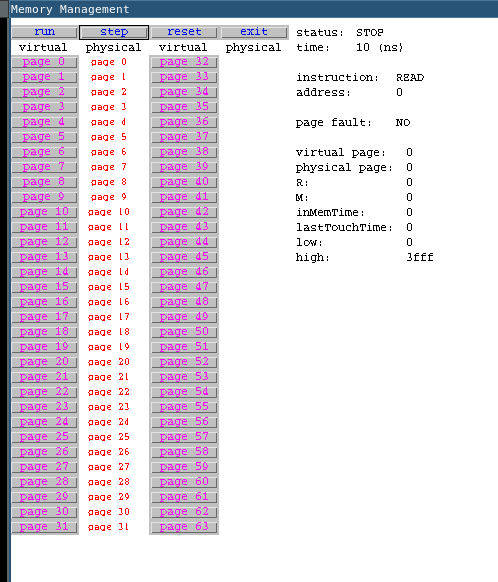
\includegraphics[width=\linewidth]{mm1}
\end{figure}
\begin{figure}[H]                  
        \caption{First step correctly mapped}
	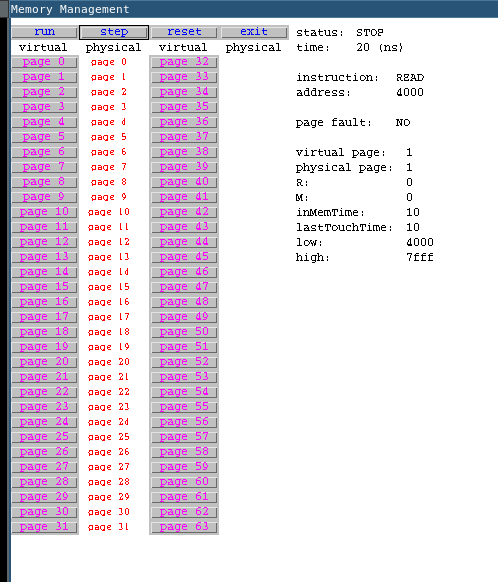
\includegraphics[width=\linewidth]{mm2}
\end{figure}     
\begin{figure}[H]
        \caption{16th page correctly mapped}                                            
	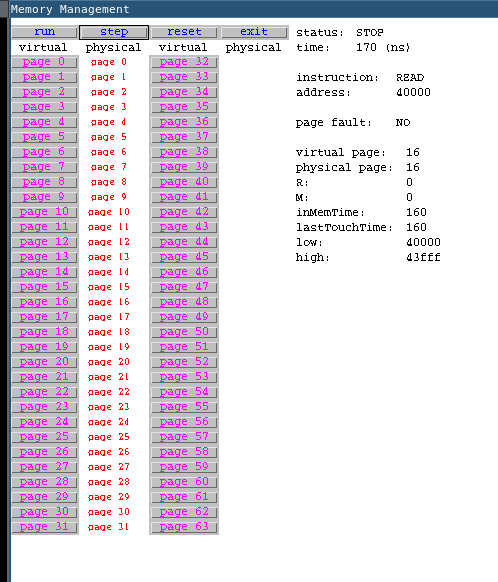
\includegraphics[width=\linewidth]{mm3}
\end{figure}
\begin{figure}[H]
        \caption{First page fault on 32th step}                                            
	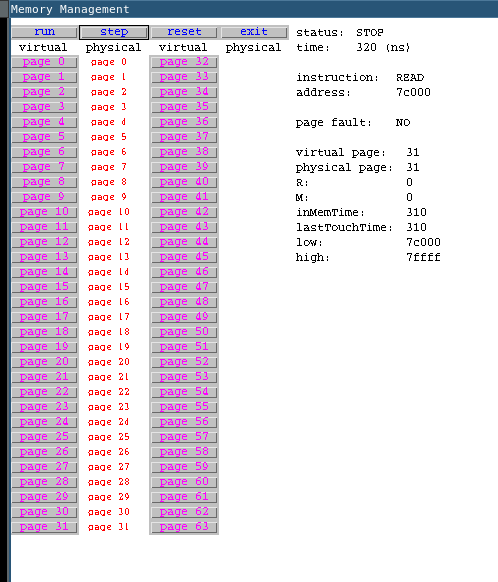
\includegraphics[width=\linewidth]{mm4}
\end{figure}
\begin{figure}[H]
        \caption{First in First out, we map page 0 physical to the page we just
	got page fault on}                                            
	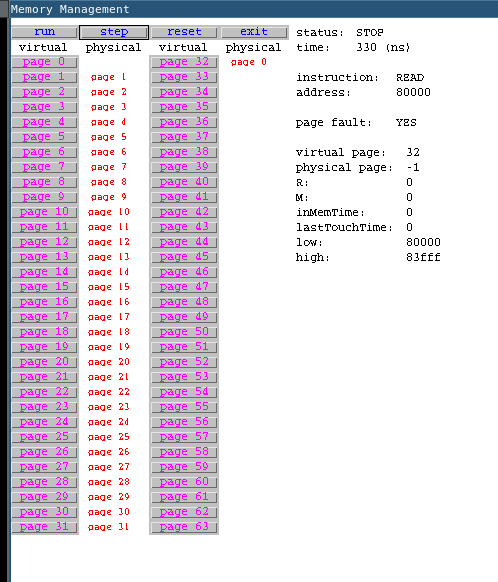
\includegraphics[width=\linewidth]{mm5}
\end{figure}
\begin{figure}[H]
        \caption{Again first in, first out}                                            
	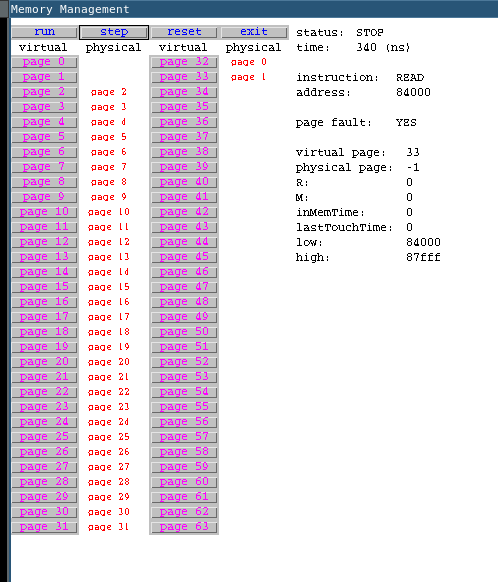
\includegraphics[width=\linewidth]{mm6}
\end{figure}
\begin{figure}[H]
        \caption{Final view of application}                                            
	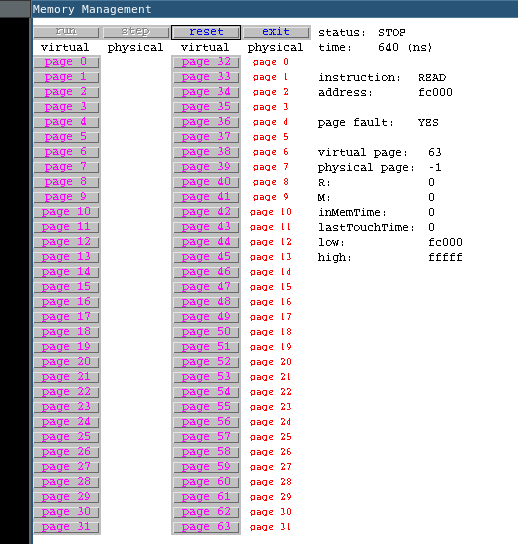
\includegraphics[width=\linewidth]{mm7}
\end{figure}
\section{Finishing comments}
Both by looking at the source code and simulation results we can say that the
simulation uses First in First out algorithm. First 8 pages were mapped
correctly because of the memory.conf file, pages up to 32 were mapped correctly
because they are mapped by default by the application. \\
Then we got page faults which were resolved by first in first out algorithm. 
\begin{thebibliography}{9}
	\bibitem{mmuWiki} \href{https://en.wikipedia.org/wiki/Memory_management_unit}{Wiki Memory Management Unit}
	\bibitem{faultWiki} \href{https://en.wikipedia.org/wiki/Page_fault}{[Wiki Page Fault]}
\bibitem{Page Replacement Algorithms}
\href{https://www.geeksforgeeks.org/page-replacement-algorithms-in-operating-systems/}{[Geeks
for Geeks page replacament algorithms]}
\bibitem{pageWiki}
\href{https://en.wikipedia.org/wiki/Page_replacement_algorithm}{Wikipedia Page
replacament algorithm}
\end{thebibliography}
\end{document}
